\section{Marco Teórico}

\subsection{Validación de Modelos}
Los modelos son representaciones matemáticas de los mecanismos que rigen los fenómenos naturales (Tedeschi, 2006) o como una construcción matemática diseñada para estudiar un sistema del mundo real o fenómeno (Giordano et al., 1997).
\vspace{.5cm}

Medina-Peralta et al. (2017) indican que la validación de un modelo en la predicción del sistema implica la comparación, por medio de algún método, de las predicciones del modelo con los valores observados del sistema real para determinar su capacidad predictiva.
\vspace{.5cm}

Mayer y Butler (1993), clasifican los métodos de validación de modelos en Evaluación Subjetiva, Técnicas Visuales, Medidas de Desviación y Pruebas Estadísticas; también señalan que debido a las complejidades y tipos de datos, no existe una combinación establecida de técnicas de validación que sea aplicable en todas las áreas.
\vspace{.5cm}

Halachmi et al. (2004), menciona que la validación determina si el modelo matemático es una representación exacta del sistema real, y una forma de validación es comparando los datos reales con los predichos por el sistema.
\vspace{.5cm}

Para la validación de un modelo se evalúan la exactitud y la precisión; la primera se refiere a la proximidad de las predicciones $( z )$  con los valores observados $( y )$, por ejemplo, sus diferencias $ ( d=y-z ) $ del cero y la segunda a la dispersión de los puntos $ (z, y) $; además, en presencia de exactitud la precisión se mide cuantificando la dispersión de dichos puntos respecto a una referencia, por ejemplo, la recta determinística  $ y=x $, o bien, evaluar la varianza de las diferencias $ (\sigma_{D}^{2}) $ alrededor del cero $ (\mu_{D}=0) $ (Medina-Peralta et al., 2017).
\vspace{.5cm}

En la Figura \ref{fig:etiqueta} se ilustra la diferencia entre la exactitud y precisión de un modelo de simulación. El caso 1 es inexacto e impreciso, el caso 2 es inexacto y preciso, el caso 3 es exacto e impreciso y el caso 4 es exacto y preciso. En un modelo de predicción lo ideal es que cumpla el caso 4. 

\begin{figure}[ht]
	\centering
	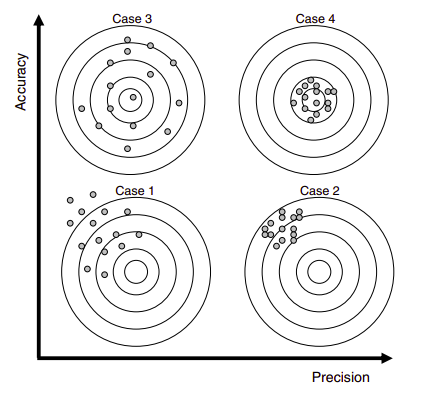
\includegraphics[width=300px]{img/tadeshi_casos.png}
	\caption{Esquematización de Exactitud y Precisión. Fuente: Tedeschi (2006).}
	\label{fig:etiqueta}
\end{figure}

\subsection{Validación de Modelos con Regresión Lineal}


\subsection{Regresión Lineal Robusta}
\subsection{Wild Bootstrap}

\subsubsection{Algoritmo de remuestreo básico}

Se asume una muestra de $ x_{1}, x_{2},  \dots,  x_{n}$ independiente e idénticamente distribuida.

\begin{enumerate}
		\item Se obtienen $B$ muestras de tamaño $n$ con reemplazo y con probabilidades iguales de la muestra original. La cardinalidad de este espacio muestra es $n^{n}$. Se denotan las muestras Bootstrap por $X^{*}_{1}, X^{*}_{2},  \dots, X^{*}_{B}$ donde cada $X^{*}_{i}$ es un vector de tamaño $n$.
		
		\item Se obtienen las muestras, $\hat{\theta}^{*}_{1} = T (X^{*}_{1}) , \hat{\theta}^{*}_{2} = T (X^{*}_{2}), \dots,\hat{\theta}^{*}_{B} = T (X^{*}_{B})$.
		
		\item Se usa la distribución empírica $\hat{F}_{\hat{\theta}^{*}}$ de la muestra $\hat{\theta}^{*}_{1},\hat{\theta}^{*}_{2},  \dots, \hat{\theta}^{*}_{B}$ para estimar $F_{\hat{\theta}} $.
\end{enumerate}

En la practica, se usa una $B$ grande para disminuir el error de simulación al evitar el calculo de todo el espacio muestra Bootstrap.

Las estimaciones para  $F_{\hat{\theta}}, \theta^{*}$ y $ \sigma_{\theta^{*}} $ están dadas respectivamente por:

\[
\hat{F}_{\hat{\theta}^{*}} \approx F_{\hat{\theta}}, 
 \hspace{.5cm} \hat{\theta}^{*} = \frac{1}{B} \sum_{i=1}^{B}  \hat{\theta}^{*}_{i} \approx \theta,
 \hspace{.5cm} Var(\hat{\theta}^{*}) = \frac{1}{B-1} \sum_{i=1}^{B}(\hat{\theta}^{*}_{i}-\hat{\theta}^{*})^2
\]


\subsubsection{Algoritmo de Remuestreo Balanceado}

Se asume una muestra  $ x_{1}, x_{2},  \dots,  x_{n}$ independiente e idénticamente distribuida y supongamos que se desean obtener $B$ muestras Bootstrap.

\begin{enumerate}
	\item  Considere el vector $ X=(x_{1}, x_{2},  \dots,  x_{n}) $.
	
	\item  Generar un vector $ N= (1,2,\dots,n,1,2,\dots,n,1,2,\dots,n)$ de longitud $nB$.
	
	\item Generar una permutación aleatoria $N^{*}$ del vector $N$.
	
	\item La muestra Bootstrap haciendo lo siguiente:
	
	$X^{*}_{1}$ =  Los elementos de $X$ comprendidos desde la primera hasta la posición $n$ de $N^{*}$.\linebreak
	$X^{*}_{2}$ =  Los elementos de $X$ comprendidos desde la posición $n + 1$ hasta la posición $2n$ de $N^{*}$.\linebreak
	.\linebreak\
	.\linebreak
	.\linebreak
	$X^{*}_{B}$ =  Los elementos de $X$  cuyas posiciones son las ultimas $n$ posiciones de $N^{*}$.
	
	\item  Se obtienen las muestras, $\hat{\theta}^{*}_{1} =T (X^{*}_{1}), \hat{\theta}^{*}_{2} =T (X^{*}_{2}), \dots, \hat{\theta}^{*}_{B} =T (X^{*}_{B})$.
	
	\item  Se usa la distribución empírica $\hat{F}_{\hat{\theta}^{*}}$ de la muestra $\hat{\theta}^{*}_{1},\hat{\theta}^{*}_{2}, \dots, \hat{\theta}^{*}_{B}$ para estimar $F_{\hat{\theta}}$
	
	
\end{enumerate}







\subsubsection{Algoritmo Bootstrap de Residuales (Rosalinda)}

Se asume que los $ \epsilon_{i} $ son independientes e idénticamente distribuidos. El algoritmo Bootstrap para generar muestras de $ R^{2} $ es el siguiente:

\begin{enumerate}
		\item Ajustar una regresión simple para el modelo $ y_{i} = \beta_{0} +\beta_{1}x_{i} + \epsilon_{i} $.
		
		\item Obtener los residuales $ \epsilon_{i} = y - \hat{y}   $
		, $i = 1,..., n $.
		
		\item  Remuestrear con probabilidades iguales la muestra $ e_{1},...,e_{n} $, para obtener $e^{*}_{11},...,e^{*}_{1n}$.
		\item Obtener $ y^{*}_{1i} = e^{*}_{1i} + \hat{y}_{1i}, i = 1, ..., n. $.
		
		\item Correr una regresión simple $ y^{*}_{1i} = \beta^{*}_{10} +\beta^{*}_{11}x_{i} + \epsilon^{*}_{1i} $ para obtener $ \hat{R}^{2*}_{1} $.
		
		\item Repetir los pasos 3 al 5, $B - 1$ veces para obtener las muestras: 
		\[
		\hat{R}^{2*}_{1} \hspace{.5cm} \hat{R}^{2*}_{2} \hspace{.5cm} \dots \hspace{.5cm} \hat{R}^{2*}_{B}
		\]
\end{enumerate}


\subsubsection{Algoritmo Bootstrap Pareado (Rosalinda)}

Supóngase que los datos surgieron de un estudio observacional donde ambas variables, $Y$ y $X$ son medidas de una colección de individuos seleccionados aleatoriamente. Supongamos que los $e_{i}$ en el modelo
$ y_{i} = \beta_{0} +\beta_{1}x_{i} + \epsilon_{i}$,    $i=1,2,..., n$ , no tienen varianza constante, lo que implica que no son idénticamente distribuidos (Givens y Hoeting, 2005; Montgomery et al., 2006).

\begin{enumerate}
	\item Considere la muestra $ w_{1} = (y_{1}, x_{1}),  w_{2} = (y_{2}, x_{2}), ..., w_{n} = (y_{n}, x_{n})$ como una muestra independiente e idénticamente distribuida donde la distribución es la conjunta $ F_{Y|X} $.
	
	\item  Tomar una muestra Bootstrap  $ w^{*}_{1}, w^{*}_{2},...,  w^{*}_{n} $ de $w_{1}, w_{2},...,  w_{n} $. Se obtienen la muestras  $y_{1}, y_{2},...,  y_{n} $ y  $x_{1}, x_{2},...,  x_{n} $.
	
	\item Correr una regresión lineal $ y^{*}_{i} = \beta_{i0} +\beta_{i1}x_{i}^{*} + \epsilon_{i} $.
	
	\item Estimar  $ \hat{R}^{2*}_{1} $.
	
	\item  Repetir los pasos 3 al 5, $B - 1$ veces para obtener las muestras: 
	\[
	\hat{R}^{2*}_{1} \hspace{.5cm} \hat{R}^{2*}_{2} \hspace{.5cm} \dots \hspace{.5cm} \hat{R}^{2*}_{B}
	\]
\end{enumerate}






\subsection{Simulación de Modelos}

\subsection{Diseño Factorial}